\chapter{Testing Framework}
\label{sec:testing}
\lettrine{A}{ll} tests performed are based on MATLAB routine executed on a Desktop PC. The images output of the thermal sensors are the result of an a priori rendering process both for the visible and the thermal case.\\
To provide a detailed overview of the testing framework, the target debris VESPA \cite{esa_vv02} is presented, describing the model used to generate the landmarks. Subsequently, the rendering tool used to generate the synthetic images is detailed. Different study cases are identified from a brief discussion on the rendered synthetic images, varying the parameters that primarily influence the sensors' output. Finally, the ground truth used for relative dynamics and the filter's figures of merit are presented. 

\section{Vega Secondary Payload Adapter}
\chaptermark{Testing Framework}
VESPA is a payload adapter that enables the Vega rocket embarking and deploying different payloads in different orbits. It was first used on Vega's second flight (VV02) in 2013, deploying the Proba-V and other two payloads in two different orbits \cite{esa_vv02}. A pre-launch picture of Proba-V mounted on VESPA is shown in \cref{fig:probavespa}.\\
\begin{figure}[H]
    \centering
    \includegraphics[width = 0.275\linewidth]{Images/Proba-V_on_Vespa_adapter_article.jpg}
    \caption{Proba-V mounted on VESPA, from \cite{esa_vv02}}
    \label{fig:probavespa}
\end{figure}

The VESPA properties are reported in \cref{tab:VESPAProp}. The VESPA debris is of interest both for the ClearSpace-1 mission \cite{biesbroek2021clearspace}, aimed to de-orbit the adapter, and for the e.Inspector mission, aimed at de-risking optical navigation technologies for uncooperative targets and collecting relevant information on the current debris status to support its removal operations. Because of its dimension, VESPA is considered an Intact Derelict Object, making its removal critical for space sustainability \cite{liou2012active}. 

\begin{table}[!h]
    \centering
    \begin{tabular}{c c c}
        Parameter & Value & Unit \\ \hline \hline 
        Payload interface diameter & 937 & \SI{}{\milli\meter} \\ \hline
        Launcher interface diameter & 2105 & \SI{}{\milli\meter} \\ \hline
        Height & 2867 & \SI{}{\milli\meter} \\ \hline
        VESPA mass & 262 & \SI{}{\kilo\gram} \\ \hline
        Maximum main payload mass & 1000 & \SI{}{\kilo\gram} \\ \hline
        Maximum secondary payload mass & 200 & \SI{}{\kilo\gram} \\ \hline
    \end{tabular}
    \caption{VESPA properties \cite{esa_vv02}}
    \label{tab:VESPAProp}
\end{table}

\subsection{VESPA wireframe model}
As specified in \cref{sec:mesmodel}, the filter uses a wireframe model of the target to compute the pseudo-measurements of the states, projecting the model features onto the image plane.\\
A STereolithograpfy File (STL) containing a detailed model of VESPA is used to define the model landmarks. As shown in \cref{fig:vespafeatures}, a landmark is generated for each face of the model. If the landmarks were to be generated from a highly detailed model (\cref{fig:vespastl}), their elevated number would compromise the filter's efficiency. For this reason, the target's original model is downscaled to avoid this issue. The detailed model, the downscaled model, and the landmarks can be observed in \cref{fig:vestastlfeat}. \\
\cref{fig:vestastlfeat} allows evaluating, it is possible to evaluate how this target might affect the navigation process: first of all, VESPA is axis-symmetrical because of its conic shape; the only elements not axis-symmetrical are the superficial elements, such as bolts or flanges. However, those present a central symmetry. This symmetry properties require to arbitrarily define which of the two identical sides of VESPA the chaser faces when the pose is initialized, as the x-y axis orientation is undefined because of the central symmetry. For the tracking, the superficial elements are the only features that could provide information about the chaser position around the axis of symmetry of VESPA.

\begin{figure}
\begin{subfigure}{0.48\linewidth}
    \centering
    \includegraphics[width =0.75\linewidth]{Images/vespina.png}
    \caption{VESPA detailed model}
    \label{fig:vespastl}
    \end{subfigure}
    \begin{subfigure}{0.48\linewidth}
    \centering
    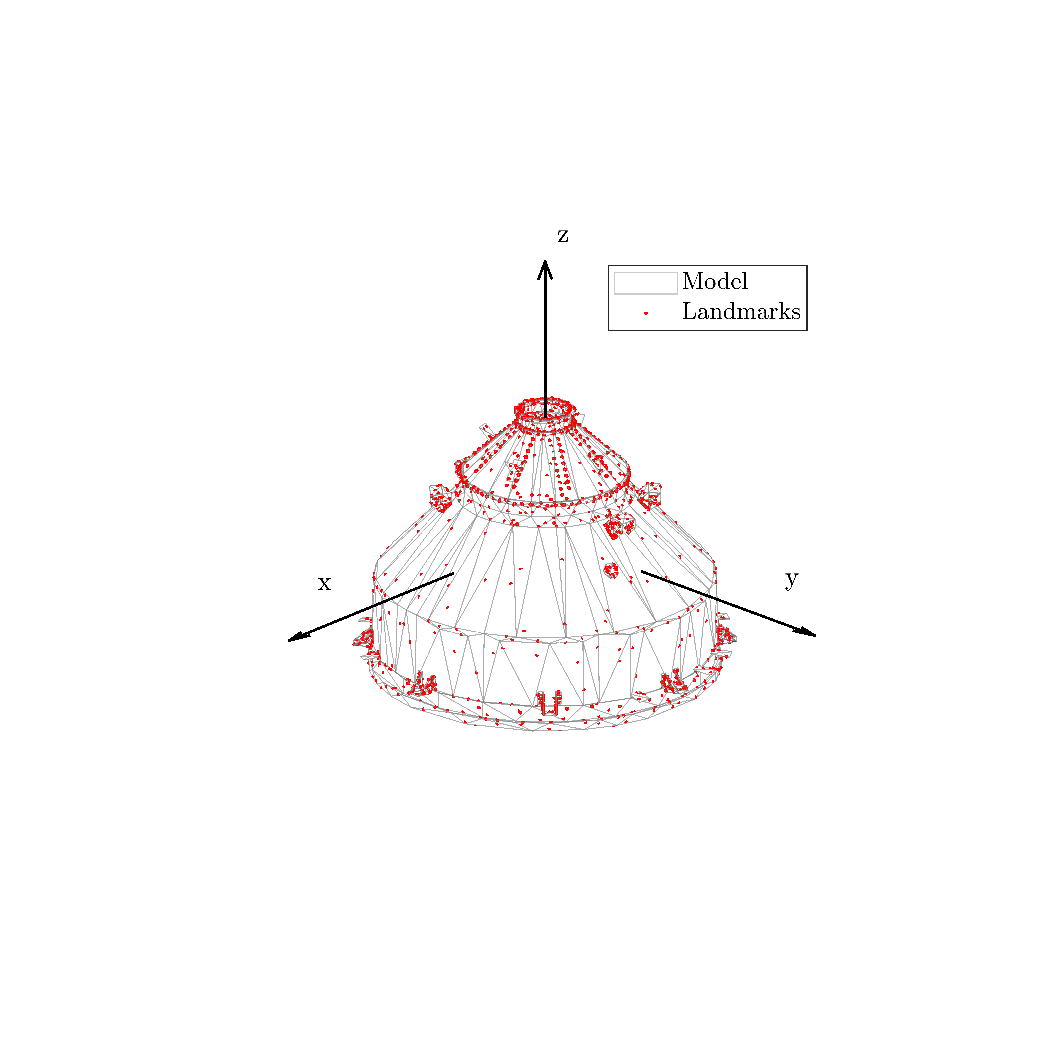
\includegraphics[clip,trim = 4cm 5cm 2.8cm 3.4cm, width =\linewidth]{Images/VESPA9mm.eps}
    \caption{VESPA downscaled model and landmarks}
    \label{fig:vespafeatures}
    \end{subfigure}
    \caption{VESPA models and generated landmarks}
    \label{fig:vestastlfeat}
\end{figure}


\section{Synthetic images rendering}
\chaptermark{Testing Framework}
\label{sec:rendering}
The visible and thermal images rendering tool was not developed or modified within the context of the thesis but was solely exploited as user. The working principle of the image generation pipeline is briefly presented, and the reader is referred to \cite{piccinin2023spacecraft} for a more detailed description. The rendering tool was initially designed for small-bodies rendering and was adapted for the space debris application for the thesis. \\
Both the VIS and TIR generation relies on Blender rendering software \cite{blender}. The process is straightforward for the visible images, as the software is intended for this task. In the case of the thermal images, a simplified thermal model of the target is used to compute the surface irradiance, which is fed into Blender to generate the thermal images. The target simplified thermal model relies on two significant assumptions. Firstly, the target thermal profile is considered spatially uniform at each given instant, so the target appearance in the thermal image is influenced only by the overall temperature, the emissivity of the different surfaces, and the view factor. Secondly, only two thermal conditions were considered: a sunlit (hot) case, which provides a bright thermal image (\cref{fig:Cas1Tir}) and an eclipse (cold) case, providing an overall darker image (\cref{fig:Cas4Tir}) assuming the target temperature close to lower limit of the sensor's sensibility. \\
The camera parameters used for the image generation are reported in \cref{tab:cams}, where it can be seen that the visible image provides a higher resolution and has a wider FOV with respect to the thermal camera.  These parameters are also used to calculate the intrinsic camera matrix to compute the filter's pseudo-measurements.\\

\begin{table}[!h]
    \begin{subtable}[h]{0.45\textwidth}
        \centering
        \begin{tabular}{l c c}
        Parameter & Value & Unit \\
        \hline \hline
        Resolution & [2000, 2000] & $\SI{}{\pixel}$ \\\hline
        FOV & [9.15, 9.15] &  $\SI{}{\deg}$\\\hline


       \end{tabular}
       \caption{VIS camera properties}
       \label{tab:viscam}
    \end{subtable}
    \hfill
    \begin{subtable}[h]{0.45\textwidth}
        \centering
        \begin{tabular}{l c c}
        Parameter & Value & Unit \\
        \hline \hline
        Resolution & [640, 512] & $\SI{}{\pixel}$ \\\hline
        FOV & [6.2, 5] &  $\SI{}{\deg}$\\\hline

        \end{tabular}
        \caption{TIR camera properties}
        \label{tab:tircame}
     \end{subtable}
     \caption{Visible and thermal camera properties}
     \label{tab:cams}
\end{table}
As environmental conditions highly influence space imagery, also the rendered images reflect this behavior. The parameters that most influence the visible and thermal images are identified to be:
\begin{itemize}
    \item the chaser-target-Sun angle $\phi \ [0 \ \pi]$ (\cref{fig:phiangle}), referred to as \textit{phase angle}, which indicates if the camera is facing the sunlit or shadowed side of the target.
    \item The \textit{elevation angle} of the chaser in the target body frame $\rho \ [-\pi/2 \ \pi/2]$ (\cref{fig:rhoangles}), that indicates in which measure the camera observes the outer or inner surface of the conical shape.
    \item The presence of eclipse.
\end{itemize}
\begin{figure}[!h]
\begin{subfigure}{0.48\linewidth}
    \centering
    \includegraphics[width=0.8\linewidth]{Images/phiangle.pdf}
    \caption{$\phi$ angle definition}
    \label{fig:phiangle}
\end{subfigure}\hfill
\begin{subfigure}{0.48\linewidth}
    \centering
    \includegraphics[width=\linewidth]{Images/rhodefinition.pdf}
    \caption{$\rho$ angle definition}
    \label{fig:rhoangles}
\end{subfigure}
    \caption{Geometrical definition of the phase angles $\phi$ and the elevation angle $\rho$}
    \label{fig:rhophi}
\end{figure}
\quad
\begin{table}[!h]
    \centering
    \begin{tabular}{p{2cm} C{2cm} C{2cm} C{2cm} C{2cm} C{3cm}}
        \multirow{2}{*}{Case} & \multirow{2}{*}{$\phi$} & \multirow{2}{*}{$\rho$} & \multicolumn{2}{c}{Target visibility} & \multirow{2}{*}{Reference figure}\\
        & & & VIS & TIR &\\\hline \hline
        A & low & high & good & good & \cref{fig:Cas1} \\ \hline
        B & low & low & poor & good & \cref{fig:Cas2}\\ \hline
        C & high & low & poor & good & \cref{fig:Cas3}\\ \hline
        D & eclipse & high & null & poor & \cref{fig:Cas4}\\ \hline
    \end{tabular}
    \caption{Different illumination cases overview}
    \label{tab:ill_cases}
\end{table}\mbox{}\\\mbox{}\\
By varying those parameters, four illumination conditions have been identified (\cref{tab:ill_cases}).\\ 
Those study cases solve the role of providing a further description of the synthetic images and provide a better understanding of the filter results in different situations.\\
\begin{itemize}
    \item \textbf{Case A} represents the most favorable illumination condition for both the visible and thermal spectra. The low phase angle provides good illumination of the target and a  high temperature that allows for a vivid thermal image (\cref{fig:Cas1Tir}). As highlighted in \cref{fig:Cas1Vis}, the high $\rho$ value results in imaging the upper side of VESPA, i.e., the outer side of its conical shape. This represents the best condition for visible imaging, as demonstrated in the second study case.
    \item \textbf{Case B} considers a low phase angle is maintained, but the elevation angle is dropped. It can be observed how observing the concavity of VESPA is critical for the visible imagery  (\cref{fig:Cas2}), as the concavity is subject to important shadows that make the target only partially visible also in good illumination conditions. The thermal image is not highly affected by the shadows, although it shall be noted that the lower side of VESPA has fewer distinguishable elements than its upper side. 
    \item \textbf{Case C} considers a situation with a low illumination condition, increasing the phase angle. As expected, even with a high $\rho$, the visible image is compromised as the target remains only partially visible (\cref{fig:Cas3}). In this condition, the thermal image is unaffected, as the rendering process works under the assumption of a uniform thermal profile. \\
    \item \textbf{Case D} investigates the eclipse condition. In that circumstance, the visible image results completely black (\cref{fig:Cas3Vis}), as the rendering process assumes the Sun as the only light source. Regarding the thermal images, it is considered the eclipse case as the cold case for the target. The sensor response was lowered to highlight a difference with the hot case, but the temperature of the target is assumed to be still within the sensor sensibility ranges (\cref{fig:Cas3Tir}). This was considered because if the target temperature were below the sensor's minimum sensibility also the thermal image would result completely black, becoming a case study not worth investigating as it would produce no results. \\
\end{itemize}
In the thesis work, the images are rendered and used without noise. For further developments, a pixel-level noise should be added to increase the realism of the testing framework \cite{BECHINI2023358}.
% The first illumination condition (case A) represents the most favorable for both the visible and thermal spectra. The low phase angle provides good illumination of the target and a  high temperature that allows for a vivid thermal image (\cref{fig:Cas1Tir}). As highlighted in \cref{fig:Cas1Vis}, the high $\rho$ value results in imaging the upper side of VESPA, i.e., the outer side of its conical shape. This represents the best condition for visible imaging, as demonstrated in the second study case.\\
% In case B (\cref{fig:Cas2}), a low phase angle is maintained, but the elevation angle is dropped. It can be observed how observing the concavity of VESPA is critical for the visible imagery, as the concavity is subject to important shadows that make the target only partially visible also in good illumination conditions. The thermal image is not highly affected by the shadows, although it shall be noted that the lower side of VESPA has fewer distinguishable elements than its upper side. 
\begin{figure}[!h]
\centering
\begin{subfigure}{0.2576\linewidth}
    \centering
    \includegraphics[width = \linewidth]{Images/Cas1Vis.png}
    \caption{VIS image}
    \label{fig:Cas1Vis}
\end{subfigure}\quad\quad\quad\quad\quad\quad\quad
\begin{subfigure}{0.32\linewidth}
    \centering
    \includegraphics[width = \linewidth]{Images/Cas1Tir.png}
    \caption{TIR image}
    \label{fig:Cas1Tir}
\end{subfigure}
\caption{Case A: low $\phi$, high $\rho$}
\label{fig:Cas1}
\end{figure}
\begin{figure}[!h]
\centering
\begin{subfigure}{0.2576\linewidth}
    \centering
    \includegraphics[width = \linewidth]{Images/Cas2Vis.png}
    \caption{VIS image}
    \label{fig:Cas2Vis}
\end{subfigure}\quad\quad\quad\quad\quad\quad\quad
\begin{subfigure}{0.32\linewidth}
    \centering
    \includegraphics[width = \linewidth]{Images/Cas2Tir.png}
    \caption{TIR image}
    \label{fig:Cas2Tir}
\end{subfigure}
\caption{Case B: low $\phi$, low $\rho$}
\label{fig:Cas2}
\end{figure}
\begin{figure}[!h]
\centering
\begin{subfigure}{0.2576\linewidth}
    \centering
    \includegraphics[width = \linewidth]{Images/Cas3Vis.png}
    \caption{VIS image}
    \label{fig:Cas3Vis}
\end{subfigure}\quad\quad\quad\quad\quad\quad\quad
\begin{subfigure}{0.32\linewidth}
    \centering
    \includegraphics[width = \linewidth]{Images/Cas3Tir.png}
    \caption{TIR image}
    \label{fig:Cas3Tir}
\end{subfigure}
\caption{Case C: high $\phi$, high $\rho$}
\label{fig:Cas3}
\end{figure}
\begin{figure}[H]
\centering
\begin{subfigure}{0.2576\linewidth}
    \centering
    \includegraphics[width = \linewidth]{Images/Cas4Vis.png}
    \caption{VIS image}
    \label{fig:Cas4Vis}
\end{subfigure}\quad\quad\quad\quad\quad\quad\quad
\begin{subfigure}{0.32\linewidth}
    \centering
    \includegraphics[width = \linewidth]{Images/eclipseTir.png}
    \caption{TIR image}
    \label{fig:Cas4Tir}
\end{subfigure}
\caption{Case D: eclipse}
\label{fig:Cas4}
\end{figure}
% In case C (\cref{fig:Cas3}), a situation with a low illumination condition is considered, increasing the phase angle. As expected, even with a high $\rho$, the visible image is compromised as the target remains only partially visible. In this condition, the thermal image is unaffected, as the rendering process works under the assumption of a uniform thermal profile. \\
% Finally, a case in eclipse is considered (case D, \cref{fig:Cas4}). In that circumstance, the visible image results completely black, as the rendering process assumes the Sun as the only light source. Regarding the thermal images, it is considered the eclipse case as the cold case for the target. The sensor response was lowered to highlight a difference with the hot case, but the temperature of the target is assumed to be still within the sensor sensibility ranges. This was considered because if the target temperature were below the sensor's minimum sensibility also the thermal image would result completely black, becoming a case study not worth investigating as it would produce no results. \\
 
\section{Reference dynamics}
\chaptermark{Testing Framework}
\label{sec:errors}
The Section discusses the reference dynamical model used to test the filter's estimation capabilities. \\
For what concerns the relative position and velocity, the chaser and the target positions are independently propagated in ECI according to a J2-perturbed Keplerian motion about the Earth. As this model of motion is well known in literature, it is not presented in the thesis. For a detailed description of this dynamics the reader is referred to \cite{alfriend2009spacecraft}. The target position is moved into the chaser LVLH frame a posteriori of the propagation. Additional orbital perturbations are not included as their effect is not appreciable in short-term propagations. \\
As far as the attitude dynamics is concerned, the target angular velocities are propagated with rigid body motion Euler's equation, assuming the principal inertia axes aligned with the body frame axes (\cref{fig:vespafeatures}). The elements of the diagonal inertia matrix were randomly defined as, for the purpose of the thesis, their physical coherence with the target's mass distribution is not relevant. As the chaser mounts two fixed cameras on its body, the cameras' z-axis is assumed to always point the center of the target body. For the sake of simplicity, both cameras are assumed to be placed in the center of the chaser body frame with the cameras' z-axis aligned with the chaser's x-axis (\cref{fig:relframes}). This results in the condition that the chaser's x axis shall always point the center of the target's body frame, as if an ideal control was applied. For this reason, the attitude of the chaser is not propagated dynamically, but by ensuring geometrically this condition along the trajectory. 
\begin{figure}[!h]
    \centering
    \includegraphics[clip, trim = 0cm 3cm 0cm 3cm, width = 0.7\linewidth]{Images/relframes.pdf}
    \caption{Schematic of the chaser, target and camera frames}
    \label{fig:relframes}
\end{figure}


\subsection{Figures of merit}
After the position and attitude are propagated according to the dynamic described in \cref{sec:errors}, and the images are rendered accordingly, the navigation filter is tested to evaluate its capability to estimate the relative pose. The criteria defined to quantitatively assess the filter's performances are:
\begin{itemize}
    \item the absolute and relative position error
    \item the attitude error
\end{itemize}
This Section defines those variables.\\
Given a simulation composed on $N$ filter updates (or equivalently $N$ measurements events) the position Absolute Knowledge Error (AKE) at a given step $i$ is defined as:
\begin{equation}
\label{eq:positionerror}
    e_{p,i} = \sqrt{(x_i -\hat{x}_i)^2 + (y_i -\hat{y}_i)^2 +(z_i -\hat{z}_i)^2 }
\end{equation}

where $\hat{\cdot}$ indicates the estimated values. \cref{eq:positionerror} can be interpreted as the distance between the true and estimated target position. The position Relative Knowledge Error (RKE) is defined as the absolute error $e_{p,i}$ normalized against the true chaser-target distance:

\begin{equation}
\label{eq:positionerrorrelative}
    e_{r,i} = \dfrac{e_{p,i}}{\sqrt{x_i^2 + y_i^2 +z_i^2 }}
\end{equation}

% \begin{equation}
% \label{eq:positionerrormean}
%     \bar{e}_p = \dfrac{1}{N}\sum_{i=1}^N e_{p,i}
% \end{equation}
% \begin{equation}
% \label{eq:positionerrorstd}
%     \sigma_{e_p} = \sqrt{\dfrac{1}{N}\sum_{i=1}^N (e_{p,i} -  \bar{e}_p)^2}
% \end{equation}
It shall be noted that this definition differs from the RKE formulation reported in the ECSS, which defines that index as the difference between the AKE and the mean of the AKE over a time interval. \\
For the attitude AKE, the Euler angle between the estimated and true relative attitude $e_{a,i}$ is computed. Initially the quaternion error is defined as:
\begin{equation}
    q_{err} = q_i \otimes \hat{q}_i'
\end{equation}
where $\hat{q}'$ is the conjugate of the estimated quaternion. The Euler angle associated with the quaternion error can be computed as
\begin{equation}
    e_{a,i} = 2\, atan2\Big(\sqrt{q_{err,1}^2 + q_{err,2}^2 + q_{err,3}^2}\ , \ q_{err,4}\Big)
\end{equation}
The Euler angle ambiguity between the clockwise or counterclockwise rotation is solved by the $atan2$ operator, which provides always the smallest between the two angles. \\
The Mean Knowledge Error (MKE) and its associated standard deviation along a simulation are generally defined according to \cref{eq:atterrormean,eq:atterrorstd}, where $e_i$ represents a generic error at at the filter step $i$.

\begin{equation}
\label{eq:atterrormean}
    \mu_{e} = \dfrac{1}{N}\sum_{i=1}^N e_{i}
\end{equation}
\begin{equation}
\label{eq:atterrorstd}
    \sigma_{e} = \sqrt{\dfrac{1}{N}\sum_{i=1}^N (e_{i} -  \mu_{e})^2}
\end{equation}

As the MKE is defined as the average of the error along the simulation, it can be computed for both the AKE and RKE. The mean of the absolute and relative errors will be referred to as Absolute MKE and Relative MKE. 